\documentclass[12pt, letterpaper,spanish]{article}
\usepackage[letterpaper]{geometry}
\usepackage[T1]{fontenc} %para escribir con caracteres utf8 como tildes
\usepackage[utf8]{inputenc} %para escribir con caracteres utf8 como tildes
\usepackage[spanish]{babel} %para escribir con caracteres utf8 como tildes
\usepackage{lmodern} % latin modern font
\usepackage{color}
\usepackage[svgnames]{xcolor} % para hacer enfasis con colores
\usepackage{amssymb}
\usepackage{amsmath}
\usepackage{hyperref}
\usepackage{multirow}
\usepackage{array}
\usepackage{mathtools} % para el modulo
\DeclarePairedDelimiter\abs{\lvert}{\rvert}%
\DeclarePairedDelimiter\norm{\lVert}{\rVert}%
\hypersetup{
	colorlinks=true,
	linkcolor=black,
	filecolor=magenta,      
	urlcolor=cyan,
}

\usepackage{listings}
\lstloadlanguages{Python}
\definecolor{background}{rgb}{0.52, 0.52, 0.51}
\definecolor{keywords}{rgb}{1.0, 0.0, 0.5}
\definecolor{comments}{rgb}{0.75, 0.75, 0.75}
\definecolor{strings}{rgb}{0.91, 0.84, 0.42}
\definecolor{names}{rgb}{0.4, 1.0, 0.0}
\definecolor{white}{rgb}{1.0, 1.0, 1.0}
\definecolor{types}{rgb}{0.13, 0.67, 0.8}
\definecolor{numbers}{rgb}{0.54, 0.17, 0.89}

\lstdefinelanguage{PySharp}{
	keywords={method, include, if, else, elif, while, continue, break, return},
	keywordstyle=\color{keywords}\bfseries,
	ndkeywords={int, void, rider, true, false},
	ndkeywordstyle=\color{types}\bfseries,
	identifierstyle=\color{white},
	sensitive=false,
	emph={print, test, example, Rossi, curves},
	emphstyle=\color{names},
	comment=[l]{//},
	morecomment=[s]{/*}{*/},
	commentstyle=\color{comments}\ttfamily,
	stringstyle=\color{strings}\ttfamily,
	morestring=[b]',
	morestring=[b]"
}

\lstset{
	language=PySharp,
	backgroundcolor=\color{background},
	extendedchars=true,
	basicstyle=\footnotesize\ttfamily,
	showstringspaces=false,
	showspaces=false,
	numbers=left,
	numberstyle=\footnotesize,
	numbersep=9pt,
	tabsize=2,
	breaklines=true,
	showtabs=false,
	captionpos=b
}


\usepackage{amsthm} % para teoremas y lemas
\usepackage{graphicx} % para imagenes
\usepackage{titling} % para el pretitle
\usepackage{clrscode3e} % para pseudocodigos
\usepackage[stable]{footmisc} % para permitir footnotes in los encabezados

%\usepackage[cache=false]{minted} %para representar los codigos necesita config extra
%\renewcommand\theFancyVerbLine{\normalsize\arabic{FancyVerbLine}} % incrementar el tamaño de linenumbers de minted


\newtheorem{theorem}{Teorema}[subsection]
\newtheorem{corollary}{Corolario}[theorem]
\newtheorem{lemma}{Lema}[subsection]
\newtheorem{lemmacorollary}{Corolario}[lemma]
\theoremstyle{definition}
\newtheorem*{definition}{Definición}
\theoremstyle{remark}
\newtheorem*{remark}{Observación}
\renewcommand{\qedsymbol}{$\blacksquare$} % se remplaza el simbolo vacio de final de demostración
\graphicspath{ {./_static/} }

%--------------------------
% NO MODIFICAR ESTE DOCUMENTO
%--------------------------
	
\begin{document}
	
\begin{titlepage}
	\begin{center}
		
\includegraphics[width = 3cm]{escudoUH} 
	\end{center}
	\begin{center}
		Universidad de La Habana \\\vspace{0.2cm} Facultad de Matemática y Computación
	\end{center}
	\centering
	\vspace{1cm} \par
	{\scshape\Large Proyecto de Compilación + Intenteligencia Artificial + Simulación\par}
	\vspace{5mm} \par
	{\scshape\Huge Simulador de un Jefe Técnico de MotoGP\par}
	\vspace{5mm} \par
	\vfill
	{\Large \textbf{Autores:} \par}
	{\large Arnel Sánchez Rodríguez \space Grupo: C312 \par}
	\href{mailto:arnelsanchezrodriguez@gmail.com}{arnelsanchezrodriguez@gmail.com}\par
	\vspace{3mm} \par
	{\large Samuel Efraín Pupo Wong \space Grupo: C312 \par}
	\href{mailto:s.pupo@estudiantes.matcom.uh.cu}{s.pupo@estudiantes.matcom.uh.cu}
	\vspace{3mm} \par
	{\large Darián Ramón Mederos \space Grupo: C312 \par}
	\href{mailto:darianrm24@gmail.com}{darianrm24@gmail.com}
	\vspace{3mm} \par
	\vfill
	{\Large 2021-2022 \par}
\end{titlepage}	
\pagebreak
\tableofcontents
\pagebreak
\section{Motociclismo de Velocidad}
	El motociclismo de velocidad es una modalidad deportiva del motociclismo disputada en circuitos de carreras pavimentados. Las motocicletas que se usan pueden ser prototipos, es decir desarrolladas específicamente para competición, o derivadas de modelos de serie (en general motocicletas deportivas) con modificaciones para aumentar las prestaciones. En el primer grupo entran las que participan en el Campeonato Mundial de Motociclismo, y en el segundo las Superbikes, las Supersport y las Superstock.
	
	Las motocicletas deben presentar una serie de características como son estabilidad, alta velocidad (tanto en recta como en paso por curva), gran aceleración, gran frenada, fácil maniobrabilidad y bajo peso.
	
	\begin{center}
		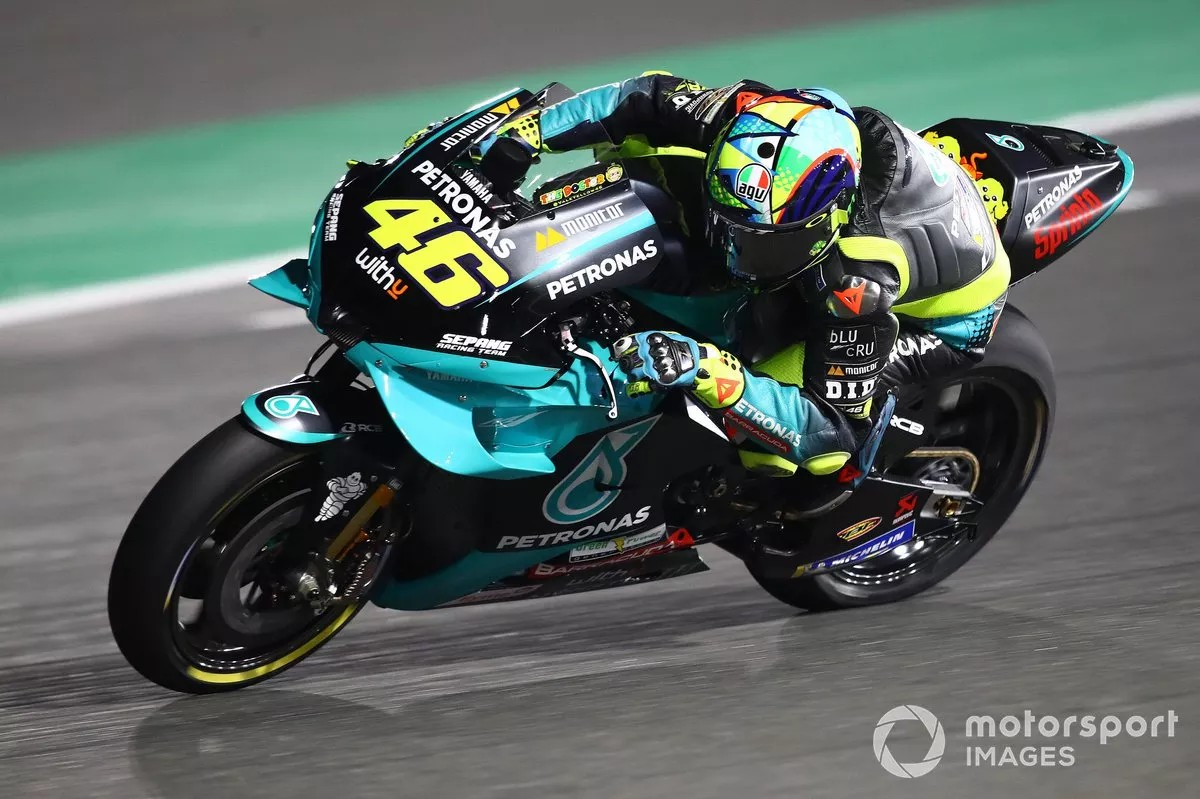
\includegraphics[width = 12cm]{imagen1} 
	\end{center}	
	
\section{Estructura del Paddock}
	El \textbf{Jefe Técnico} de cada estructura se configura como una personalidad de bastante importancia dentro de un box, pues es quién se encarga de dirigir y controlar que todo funcione como un excelente engranaje que gane carreras. De igual importancia es la telemetría dentro de un box en MotoGP. Al fin y al cabo, los \textbf{Ingenieros Telemétricos} son las personas que se encargan de analizar, leer y comprender todos los datos proporcionados por el piloto, así como transmitirselos en boca al protagonista. Se trata de una figura de la que depende mucha de la información acerca de cualquier cambio realizado en la moto o asumir los puntos más fuertes de sus pilotos. Los \textbf{Mecánicos} también desempeñan un papel fundamental a la hora de construir la máquina perfecta.

\section{Pista}
	Se utilizará como referencia el circuito de Misano, Misano World Circuit Marco Simoncelli, autódromo localizado en la fracción de Santa Mónica, comuna de Misano Adriático (provincia de Rímini), región de Emilia-Romaña, Italia. 
	
	\begin{center}
		\includegraphics[width = 12cm]{circuito} 
	\end{center}
	
\section{Definición del Problema}
	Existirán varios pilotos con sus respectivas motos, las cuáles difieren entre sí en cuanto a sus prestaciones. Cada piloto posee su propio método de manejo, siendo algunos más cuidadosos y otros más agresivos. La pista se encuentra influenciada por el accionar del clima, puesto que no es lo mismo el manejo durante un día soleado que bajo la lluvia. Por tanto, el resultado de un piloto se verá condicionado por su moto, su modo de conducción y el clima.\par
	Sin embargo, durante la carrera las condiciones pueden variar y es necesario realizar los ajustes necesarios para que el piloto mejore su rendimiento, los cuales se harán al pasar de una seccion a otra de la pista o al finalizar cada vuelta. Esto podrá hacerse utilizando un lenguaje imperativo, mediante el uso de palabras claves para que el piloto no necesite analizar situaciones complejas y pueda concentrarse en pilotar de la forma mas eficiente posible.\par
	De esta manera, la simulación de la carrera será dinámica, puesto que entre las vueltas podrán existir variaciones provocadas por los ajustes propuestos por el Jefe Técnico, el cuál podrá ser una persona o una IA.\par
	
\section{Definición del Lenguaje}
	\subsection{Introducción a PySharp (P\#)}
	\subsubsection{Hello world!}
	
	\begin{lstlisting}[language={PySharp}]
		method void main() {
			print("Hello World!");
		}
	\end{lstlisting}	
	Los archivos de P\# suelen tener la extensión de archivo .pys.\par
	
	\subsubsection{Estructura del Programa}
	Los conceptos organizativos clave en P\# son programas, tipos y miembros. Los programas P\# constan de un archivo fuente. Los programas declaran tipos y miembros. Las motocicletas y los motociclistas son ejemplos de tipos. Los métodos y propiedades son ejemplos de miembros.
	
	\subsubsection{Tipos y Variables}
	En P\# solo existen tipos de valor, no hay de referencia. Por tanto, todas las variables contienen directamente sus datos, cada una tiene su propia copia y no es posible que las operaciones en una afecten a otra.\par
	\begin{center}
		\begin{tabular}{| c | c | m{5cm} | }
			\hline
			Categoría & Tipo & Descripción \\ \hline
			\multirow{5}{*}{Tipos} & \multirow{4}{*}{Tipos Simples} & Entero con signo: int \\ \cline{3-3}
			&  & Punto flotante IEEE: double \\ \cline{3-3}
			&  & Booleanos: bool \\ \cline{3-3}
			&  & Cadenas Unicode: string \\ \cline{2-3}
			& Tipos que aceptan valores NULL & Extensiones de todos los demás tipos de valor con un valor nulo \\ \hline
		\end{tabular}
	\end{center}
	\subsubsection{Expresiones}
	Las expresiones se construyen a partir de operandos y operadores. Los operadores de una expresión indican qué operaciones aplicar a los operandos. Los ejemplos de operadores incluyen +, -, * y /. Los ejemplos de operandos incluyen literales, variables y expresiones.\par
	\begin{center}
		\begin{tabular}{| c | c | m{5cm} | }
			\hline
			Categoría & Expresión & Descripción \\ \hline
			\multirow{2}{*}{Primaria} & x(...) & Invocación de método \\ \cline{2-3}
			& x[...] & Acceso a matrices e indexadores \\ \hline
			\multirow{3}{*}{Unaria} & +x & Identidad \\ \cline{2-3}
			& -x & Negación \\ \cline{2-3}
			& !x & Negación lógica \\ \hline
			\multirow{4}{*}{Multiplicativa} & x * y & Multiplicación \\ \cline{2-3}
			& x / y & División \\ \cline{2-3}
			& x \% y & Resto \\ \cline{2-3} 
			& x ** y & Exponenciación \\ \hline
			\multirow{2}{*}{Aditiva} & x + y & Adición y concatenación de strings \\ \cline{2-3}
			& x - y & Substracción \\ \hline
			\multirow{4}{*}{Relacionales} & x < y & Menor que \\ \cline{2-3} 
			& x > y & Mayor que \\ \cline{2-3}
			& x <= y & Menor o igual que \\ \cline{2-3} 
			& x >= y & Mayor o igual que \\ \hline
			\multirow{2}{*}{Igualdad} & x == y & Igual \\ \cline{2-3} 
			& x != y & Distinto \\ \hline 
			Condicionales AND & x \&\& y & Evalúa y si y sólo si x es verdadera \\ \hline
			Condicionales OR & x || y & Evalúa y si y sólo si x es falsa \\ \hline
			Condicionales XOR & x \textasciicircum{} y & \\ \hline
			\multirow{2}{*}{Asignación} & x = y & Asignación \\ \cline{2-3}
			& x op= y & Asignación compuesta; los operadores admitidos son *= /= \%= **= += -= \&\&= ||= \textasciicircum{}= \\ \hline
		\end{tabular}
	\end{center}
	\subsubsection{Declaraciones}
	Las acciones de un programa se expresan mediante declaraciones. P\# admite varios tipos diferentes de declaraciones, algunas de las cuales se definen en términos de declaraciones integradas.
	
	Un \textbf{bloque} permite escribir múltiples declaraciones en contextos donde se permite una sola declaración. Un bloque consta de una lista de declaraciones escritas entre los delimitadores\{y\}.
	
	Las sentencias de \textbf{declaración} se utilizan para declarar variables, valga la redundancia.
	
	\begin{lstlisting}[language={PySharp}]
		method void example() {
			int a = 1;
		}
	\end{lstlisting}
	
	Las \textbf{declaraciones de expresión} se utilizan para evaluar expresiones. Las expresiones que se pueden usar como declaraciones incluyen invocaciones de métodos, asignaciones que usan = y los operadores de asignación compuesta.
	
	\begin{lstlisting}[language={PySharp}]
		method void example() {
			int a = 1;
			print(a + 2);
		}
	\end{lstlisting}
	
	La \textbf{instrucción de selección} se utiliza para seleccionar una de varias declaraciones posibles para su ejecución en función del valor de alguna expresión. Este es el caso de la sentencia \textbf{if}.
	
	\begin{lstlisting}[language={PySharp}]
		method void example(int a) {
			if (a < 5) {
				print(a);
			}
			else {
				print(a % 5);
			}
		}
	\end{lstlisting}
	
	La \textbf{instrucción de iteración} se utiliza para ejecutar repetidamente una instrucción incorporada. Este es el caso de la instrucción \textbf{while}.
	
	\begin{lstlisting}[language={PySharp}]
		method void example(int a) {
			while (a > 5) {
				print(a);
				a -= 1;
			}
		}
	\end{lstlisting}
	
	Las \textbf{sentencias de salto} se utilizan para transferir el control. En este grupo están las declaraciones de \textbf{break}, \textbf{continue} y \textbf{return}.
	
	\begin{lstlisting}[language={PySharp}]
		method int example() {
			while (true) {
				x = input()
				if (x == "x") {
					continue;
				}
				elif (x == "") {
					break;
				}
				print(x);
			}
			return 0;
		}
	\end{lstlisting}
	
	\subsubsection{Tipos especiales}
	Los \textbf{tipos especiales} son los elementos más importantes de P\#, constituyen estructuras de bloques compuestas por acciones (métodos). Un tipo proporciona una definición para casos de, por ejemplo, motociclistas o motocicletas. Su declaración comienza con un encabezado que especifica qué tipo se va a crear y el nombre que se le dará a esta instancia. El encabezado va seguido del cuerpo del tipo, que consiste en una lista de declaraciones de miembros escritas entre los delimitadores\{y\}.
	
	\begin{lstlisting}[language={PySharp}]
		rider Rossi() {
			method int example() {    
				return 0;
			}
			
			method void curves() {    
				...
			}
			...
		}
	\end{lstlisting}
	\subsubsection{Métodos}
	Un \textbf{método} es un miembro que implementa un cálculo o acción que se puede realizar por tipo. Los métodos tienen una lista (posiblemente vacía) de \textbf{parámetros}, que representan valores o referencias de variables pasadas al método, y un tipo de retorno, que especifica el tipo de valor calculado y devuelto por el método. El tipo de retorno de un método es nulo si no devuelve un valor.
	
	\subsubsection{Parámetros}
	Los \textbf{parámetros} se utilizan para pasar valores o referencias de variables a métodos. Los parámetros de un método obtienen sus valores reales de los \textbf{argumentos} que se especifican cuando se invoca el método. Las modificaciones de un valor de parámetro no afectan el argumento que se pasó para el parámetro.
	
	\subsubsection{Cuerpo del método y variables locales}
	El cuerpo de un método especifica las declaraciones que se ejecutarán cuando se invoca el método. El cuerpo de un método puede declarar variables que son específicas de la invocación del método. Estas variables se denominan variables locales. Una declaración de variable local especifica un nombre de tipo, un nombre de variable y un valor inicial.
	
	\subsubsection{Operadores}
	Un \textbf{operador} es un miembro que define el significado de aplicar un operador de expresión particular. Se pueden definir solamente operadores binarios.\par
	
	\textbf{Operadores Binarios:}
	\begin{lstlisting}[language={PySharp}]
		3+5;
		true && false;
	\end{lstlisting}
	
	\subsubsection{Análisis Léxico}
	\textbf{input}\par
	: input\_element* new\_line\par
	| directive\par
	;\par
	
	\textbf{input\_element}\par
	: whitespace\par
	| comment\par
	| token\par
	;\par
	
	\underline{\textbf{Terminadores de línea}}\par
	\textbf{new\_line}\par
	: '<Caracter de retorno (U+000D)>'\par
	| '<Caracter de avance de línea (U+000A)>'\par
	;\par
	
	\textbf{whitespace}\par
	: '<Cualquier personaje con clase Unicode Zs>'\par
	| '<Caracter de tabulación horizontal (U+0009)>'\par
	;\par
	
	\underline{\textbf{Comentarios}}\par
	\textbf{comment}\par
	: '\#' comment\_section '\#'\par
	;\par
	
	\underline{\textbf{Tokens}}\par
	\textbf{token}\par
	: identifier\par
	| keyword\par
	| literal\par
	| operator\_or\_punctuator\par
	;\par
	
	\underline{\textbf{Identificadores}}\par
	\textbf{identifier}\par
	: '<Un identificador que no es una palabra clave>'\par
	| identifier\_start\_character identifier\_part\_character*\par
	;\par
	
	\textbf{identifier\_start\_character}\par
	: letter\_character\par
	| '<Caracter guión bajo (U+005F)>'\par
	;\par
	
	\textbf{identifier\_part\_character}\par
	: letter\_character\par
	| decimal\_digit\par
	| '<Caracter guión bajo (U+005F)>'\par
	;\par
	
	\textbf{letter\_character}\par
	: uppercase\_letter\_character\par
	| lowercase\_letter\_character\par
	;\par
	
	\textbf{uppercase\_letter\_character}\par
	: 'A' | 'B' | 'C' | 'D' | 'E' | 'F' | 'G' | 'H'\par 
	| 'I' | 'K' | 'L' | 'M' | 'N' | 'O' | 'P' | 'Q'\par 
	| 'R' | 'S' | 'T' | 'V' | 'X' | 'Y' | 'Z'\par    
	;\par
	
	\textbf{lowercase\_letter\_character}\par
	: 'a' | 'b' | 'c' | 'd' | 'e' | 'f' | 'g' | 'h'\par 
	| 'i' | 'k' | 'l' | 'm' | 'n' | 'o' | 'p' | 'q'\par
	| 'r' | 's' | 't' | 'v' | 'x' | 'y' | 'z'\par
	;\par
	
	\textbf{decimal\_digit}\par
	: '0' | '1' | '2' | '3' | '4'\par 
	| '5' | '6' | '7' | '8' | '9'\par
	;\par
	
	\underline{\textbf{Palabras Claves}}\par
	\textbf{keyword}\par             
	: 'bool'\par
	| 'break'\par
	| 'continue'\par 
	| 'double'\par
	| 'elif'\par
	| 'else'\par
	| 'false'\par
	| 'if'\par
	| 'int'\par
	| 'method'\par
	| 'null'\par
	| 'return'\par
	| 'string'\par
	| 'true'\par
	| 'void'\par
	| 'while'\par
	
	| 'bike'\par
	| 'rider'\par
	
	| 'brakes'\par
	| 'max\_speed'\par
	| 'weight'\par
	| 'chassis\_stiffness'\par
	| 'speed'\par
	| 'tyres'\par
	| 'cornering'\par
	| 'step\_by\_line'\par		
	;\par
	
	\underline{\textbf{Literales}}\par
	\textbf{literal}\par
	: boolean\_literal\par
	| integer\_literal\par
	| double\_literal\par
	| string\_literal\par
	| null\_literal\par
	;\par
	
	\underline{\textbf{Literales Booleanos}}\par
	\textbf{boolean\_literal}\par
	: 'true'\par
	| 'false'\par
	;\par
	
	\underline{\textbf{Literales Enteros}}\par
	\textbf{integer\_literal}\par
	: decimal\_digit\par
	;\par
	
	\underline{\textbf{Literales flotantes}}\par
	\textbf{double\_literal}\par
	: decimal\_digit+ '.' decimal\_digit+\par
	;\par
	
	\underline{\textbf{Literales de Cadenas}}\par
	\textbf{string\_literal}\par
	: '\"' string\_literal\_character* '\"'\par
	;\par
	
	\textbf{string\_literal\_character}\par
	: '<Cualquier caracter, excepto " (U+0022)'\par
	;\par
	
	\underline{\textbf{Literales Nulos}}\par
	\textbf{null\_literal}\par
	: 'null'\par
	;\par
	
	\underline{\textbf{Operadores y signos de puntuación}}\par		
	\textbf{operator\_or\_punctuator}\par
	: '\{' \par
	| '\}' \par
	| '[' \par
	| ']' \par
	| '(' \par
	| ')' \par
	| '.' \par
	| ',' \par  
	| ':' \par
	| ';' \par
	| '+' \par
	| '-' \par
	| '*' \par
	| '/' \par
	| '\%' \par
	| '**' \par
	| '=' \par
	| '<' \par
	| '>' \par
	| '\&\&' \par
	| '||' \par
	| '==' \par
	| '!=' \par
	| '<=' \par
	| '>=' \par
	| '+=' \par
	| '-=' \par
	| '*=' \par
	| '/=' \par
	| '\%=' \par
	| '**=' \par
	| '\&\&=' \par
	| '||=' \par
	| '\textasciicircum{}=' \par
	;\par
	\underline{\textbf{Directivas}}\par
	\textbf{directive}\par
	: 'include' '<Nombre\_del\_archivo.pys>' ';'\par
	;\par
	
	\subsection{Explicación de la Implementación}
	Para crear nuestra gramatica nos apoyamos en los lenguajes Python y CSharp , de ahi el nombre de nuestro DSL PySharp.
	
	Cuando se recibe el código se tokeniza, luego de tener los tokens resultantes acordamos que tendríamos como una línea e implementamos el método $split_linese$ , el cual	recibe los tokens y los convierte en líneas , estas líneas son pasadas al parser.
	
	El parser que decidimos desarrolar fue el parser LL , lo primero que hicimos fue las producciones , donde decidimos como serían correctas
	sintácticamente nuestras líneas, las producciones generan todas las posibles cadenas válidas para nuestro lenguaje y no existen cadenas
	que son generadas por nuestra gramática que no pertenezcan a nuestro lenguaje. De esta forma con una gramática válida empezamos al proceso
	de parsing. Nuestro parser necesita un método $hacer_first$ primeramente para hacer los first de cada cadena posible de nuestra gramática,
	luego llamamos un método auxiliar $calcular_first_restantes$ el cual tiene la función de calcular los first de los no terminales que aún
	no lo tienen calculado , nos hace falta guardar los first de los no terminales pq los necesitamos para hallar los follows en el método
	$hacer_follow$ .Luego de invocar a $hacer_follow$ debemos invocar un metodo auxiliar $completar_follows$ el cual se encarga de satisfacer
	la regla de los follows que dice que el follow de la cabeza de la producción es subconjunto del follow del último no terminal , si el último no terminal puede ser el último elemento de la producción.
	
	Teniendo los first y los follows construimos la tabla LL(1) mediante el metodo $construir_tabla_LL$ , al tener la tabla ya podemos comprobar que nuestra gramática no es ambigua , siempre existe solo una producción que aplicar. Luego creamos el metodo parsear al que hay que pasarle	todas las líneas de nuestro código una por una y este realiza la comprobacion sintáctica y en este mismo método vamos a ir creando nuestro	$AST$ para luego hacer el chequeo semántico. Para crear el $AST$ utilizamos metodos como $CreaNododExpresion$, $CreaNodoCondicion$, $CreaNododFuncion$, $EligeTipoDdeclaracion$, entre otros, declarados en la clase Parser. 
	
	Nuestro AST tiene un nodo por cada declaración que se puede realizar en el código. Tiene un nodo para una definición de función, una 
	definición de variables, redefinición de variables, If, WHile, Rider, Bike, Return. En cada uno de estos nodos excepto Rider y Bike sí existe un ámbito como es el caso del nodo If, el While y la definición de función, cada uno de estos nodo tiene como atributo un tipo de nodo Program, el cuál posee una lista de declaraciones y por lo tanto en él se pueden guardar la lista de declaraciones que se haga en el ámbito.
	
	Explicada la estructura del AST pasamos al chequeo semántico sobre este. Hacemos 3 recorridos sobre el AST, el primero para validar cada nodo. Un nodo es válido si todo lo que tiene guardado en sus atributos que es dependiente del contexto puede ser utilizado desde ese contexto y de la forma que se quiere. Decimos esto porque por ejemplo las variables solo se pueden redefinir en el contexto en que fueron definidas. Decir que cada vez que creamos una función o un tipo creamos un contexto que responde a dicho ámbito. Todo lo que se defina en dicho ámbito pertenece a su contexto, no importa si se define dentro de un While o dentro de un If. En resumen los contextos en nuestro programa funcionan como en python con la particularidad de que no tenemos variables globales, si quieres redefinir una variable debes hacerlo en el contexto donde fue definida y solo se crea un nuevo contexto cuando se crea una funcion fuera de un tipo o cuando se crea un tipo. Destacar que las funciones definidas dentro de los tipos solo tienen el mismo context, y no se le pueden pasar parámetros.
	
	Volviendo al AST, hacemos una segunda pasada, en esta pasada verificamos los tipos donde en los nodos en que hay expresiones inducimos el tipo. Decir que	una expresión para nosotros puede ser una expresión aritmética , un bool, o un string, podemos incluir variables y llamado a función. La tercera pasada la hacemos para evaluar nuestros nodos. Si encontramos un nodo $Def_Fun$ no lo evaluamos, una definición de función se evalua cuando se llama a la función.
	
	Cuando se crea un tipo se importan las variables que puede tener ese tipo en la simulación, dentro de un tipo Bike solo se puede redefinir una función , la función $select_configuration$ que debe ser void , aunque dentro de la funcion si se pueden redefinir las variables de Bike, en este caso el objetivo de $select_configuration$ es seleccionar el tipo de gomas dadas las características de la moto y el ambiente y por tanto modificar la variable tires del contexto del tipo, la cuál utilizará el simulador. 
	
	Dentro de un tipo Rider existen en el contexto, igual que en Bike, variables que pertenecen a Rider que fueron importadas desde la simulación, en este caso se pueden redefinir dos de ellas $cornering$ y $step_by_line$ que posteriormente serán pasadas al simulador, estas variables tienen mucha influencia en la simulación ya que son la habilidad en recta y en curva de un piloto. Son variables enteras que lo maximo que pueden ser es 10 , en caso de que se entre un valor mayor se supondra que se quiso entrar el maximo de habilidad y la variable será igual a 10 .En cuanto a las funciones se podrán definir $select_action$ que debe retornar un valor entero y es la encargada
	de elegir que acción realizar, para hacer este metodo podemos tener en cuenta las características del piloto que pueden ser llamadas y están actualizadas. También podemos definir la funcion $select_acceleration$ la cual debe ser void y su función debe ser actualizar la aceleracion de un agente.
	
	\subsection{Conexion Simulacion - Compilacion}
	
	El resultado del DSL si se hacen los 3 recorridos del AST sin error, son dos listas, una con todos los pilotos que fueron creados y otra con todas las motos , a partir de estas listas se crean los pilotos y las motos en la simulacion. En la simulacion los pilotos que no fueron creados en el código ejecutan sus métodos como normalmente, en el caso de un piloto que fue creado desde el DSL se ejecuta la función definida en el DSL, pero antes de ejecutarla se actualiza el contexto de la funcion para que dicha función pueda apoyarse en la situación actual. Luego de la ejecución de la función dependiendo que función se ejecutó se importa a la simulación la variable que se quiere desde el contexto del método. 		
	
	
\section{Simulación}
	Primeramente nos propusimos simular una carrera de MotoGP contrareloj, luego de que tenemos los agentes(un agente es una tupla moto-piloto) y el ambiente(un ambiente es una tupla clima-pista) generados se simula cada sección de la pista, se calcula la influencia que ejerce el ambiente sobre el agente y las propias interacciones del agente consigo mismo, el tiempo que le demora a cada piloto en circular dicha sección de la pista y la aceleración y la acción que escogerá dicho piloto en esa sección, ya sea mediante una función redefinida desd el DSL o por una Inteligencia Artificial.
	
	\subsection{Clima}
	En cada sección de la pista se hacen pequeñas variaciones a los parámetros del clima, pero no al estado del clima, para darle un poco más de complejidad al sistema, luego de cada vuelta sí se modifica completamente el estado del clima y sus parámetros. Las simulaciones del clima se realizan mediante la distribución normal, que nos permite generar una variable aleatoria pero sin cambios tan bruscos en el promedio de sus casos.
	
	\subsection{Interacciones}
	Como habíamos mencionado existen varias interacciones entre un agente y un ambiente y dentro de un propio agente:
	\begin{itemize}
		\item Si la temperatura baja se enfrían los neumáticos y se pierde adherencia al pavimento
		\begin{itemize}
			\item Disminuye el paso por curva
			\item Disminuye el paso por recta
			\item Aumenta la probabilidad de caerse de la moto
		\end{itemize} 
		\item Si la temperatura aumenta se calientan los neumáticos y se gana adherencia al pavimento, se desgastan más rápido
		\begin{itemize}
			\item Aumenta el paso por curva
			\item Aumenta el paso por recta
			\item Disminuye la probabilidad de caerse de la moto
			\item Aumenta la probabilidad de romper el motor de la moto
			\item Aumenta la probabilidad de reventar los neumáticos de la moto
		\end{itemize}
		\item Si la visibilidad baja
		\begin{itemize}
			\item Disminuye el paso por curva
			\item Disminuye el paso por recta
			\item Aumenta la probabilidad de caerse de la moto
		\end{itemize}
		\item Si la visibilidad aumenta
		\begin{itemize}
			\item Aumenta el paso por curva
			\item Aumenta el paso por recta
			\item Disminuye la probabilidad de caerse de la moto
		\end{itemize}
		\item Si la humedad aumenta se pierde adherencia al pavimento
		\begin{itemize}
			\item Disminuye el paso por curva
			\item Disminuye el paso por recta
			\item Aumenta la probabilidad de caerse de la moto
		\end{itemize}
		\item Si la humedad baja se gana adherencia al pavimento
		\begin{itemize}
			\item Aumenta el paso por curva
			\item Aumenta el paso por recta
			\item Disminuye la probabilidad de caerse de la moto
		\end{itemize}
		
		\item Si el viento de de frente
		\begin{itemize}
			\item Disminuye el paso por curva
			\item Disminuye el paso por recta
			\item Aumenta la probabilidad de reventar los neumáticos de la moto
		\end{itemize}
		\item Si el viento de de espaldas
		\begin{itemize}
			\item Aumenta el paso por curva
			\item Aumenta el paso por recta
			\item Aumenta la probabilidad de caerse de la moto
			\item Aumenta la probabilidad de romper el motor de la moto
		\end{itemize}
		\item Si el viento de de lado
		\begin{itemize}
			\item Aumenta el paso por curva
			\item Aumenta el paso por recta
			\item Aumenta la probabilidad de caerse de la moto
		\end{itemize}
		
		\item Si el estado del clima es soleado aumenta la temperatura
		\item Si el estado del clima es lluvioso aumenta la humedad
		\item Si el estado del clima es nublado condiciones perfectas para correr
		
		\item Si disminuye la rigidez del chasis tiene más torsión
		\begin{itemize}
			\item Aumenta el paso por curva
			\item Disminuye el paso por recta
		\end{itemize}
		\item Si aumenta la rigidez del chasis tiene menos torsión
		\begin{itemize}
			\item Disminuye el paso por curva
			\item Aumenta el paso por recta
		\end{itemize}
		
		\item Si disminuye la frenada se frena en más distancia
		\begin{itemize}
			\item Aumenta el paso por curva
			\item Disminuye el paso por recta
		\end{itemize}
		\item Si aumenta la frenada se frena en menos distancia
		\begin{itemize}
			\item Disminuye el paso por curva
			\item Aumenta el paso por recta
		\end{itemize}
	\end{itemize}
	De acuerdo a las interacciones anteriores se debe escoger el neumático lo más preciso posible y este provocará una combinación entre estos factores.

\section{Inteligencia Artificial}
	Como nuestro proyecto se basa en simular una carrera de MotoGP donde hay n corredores, aquellos que no hayan sido diseñados mediante DSL son controlados por IA, el comportamiento de la cual varía a partir de las condiciones del ambiente que lo rodea, las características de su moto y la experiencia del propio piloto.
	
	Para la implementación de la IA se utilizan Sistemas Expertos generados mediante el uso de un procedimiento declarativo/imperativo, apoyándonos en la biblioteca PyKE de Python.
	
	Se emplea como base de conocimiento el conjunto de variables que forman parte de la simulación y que influyen en su desempeño, como:
	\begin{itemize}
		\item las características de la moto (velocidad, frenos, chasis)
		\item el estado del clima (soleado, nublado o lluvioso)
		\item la intensidad y el sentido del viento
		\item la humedad y la temperatura del ambiente
		\item la sección de pista que se está corriendo (curva o recta)
		\item la velocidad máxima alcanzable en la sección
		\item las habilidades del piloto (en rectas y curvas)
		\item entre otros
	\end{itemize}
	
	\subsection{Configuración de la moto}
	La primera heurística es la encargada de escoger la mejor configuración de la moto. De este modo, atendiendo a las condiciones iniciales de la carrera (que serán los hechos), la IA podrá tomar decisiones atendiendo a las reglas definidas. Al ser declarativas, las determinaciones tomadas se obtendrán mediante match hechos-reglas.
	Los hechos del sistema se presentan mediante una lógica difusa y son procesados para ser analizados:
	\begin{lstlisting}[language={PySharp}, label={Script}]
		rainy(True)
		humidity(False)
		windy(False)
		wind_direction(2)
	\end{lstlisting}
	
	Las reglas del sistema se formulan del modo:
	\begin{lstlisting}[language={PySharp}, label={Script}]
		soft
		use select_tires(0)
		when
		moto_facts.windy(True)
		moto_facts.wind_direction(3)
		
		medium_1
		use select_tires(1)
		when
		moto_facts.windy(False)
		
		medium_2
		use select_tires(1)
		when
		moto_facts.windy(True)
		moto_facts.wind_direction(2)
		
		hard
		use select_tires(2)
		when
		moto_facts.windy(True)
		moto_facts.wind_direction(1)
	\end{lstlisting}
	
	Luego, consultando los resultados obtenidos por las librerías de PyKE, mediante Python de manera imperativa será posible la interacción de la estructura antes expuesta con la simulación de la carrera.
	Atendiendo al ejemplo mostrado de selección de gomas, el sistema declarativo de PyKE devuelve el cálculo de una ecuación:
	$$valor_tipo_goma + valor_goma = selección$$
	
	El resultado obtenido se utiliza para generar el tipo de las gomas seleccionadas, mediante el uso de un Enum en Python:
	\begin{lstlisting}[language={Python}, label={Script}]
		class Tires(Enum):
		Slick_Soft = 0
		Slick_Medium = 1
		Slick_Hard = 2
		Rain_Soft = 3
		Rain_Medium = 4
	\end{lstlisting}
	
	\subsection{Selección de acciones}
	Una segunda heurística será la encargada de escoger la acción que debe ejecutar el piloto, atendiendo a las condiciones de la carrera:
	\begin{itemize}
		\item aumentar/disminuir/mantener velocidad
		\item doblar
		\item ir a los pits
		\item combinaciones de todas las anteriores
	\end{itemize}
	(Ejemplo: aumentar velocidad + doblar + ir a los pits)
	
	En este caso, se utiliza el mismo método expuesto en la configuración de la moto: declarativo/imperativo con el uso de PyKE.
	Se analizan los parámetros de velocidad, sección de la pista y estado del clima:
	\begin{lstlisting}[language={PySharp}, label={Script}]
		speed(3)
		curve(False)
		tires(False)
		rainy(True)
		humidity(False)
	\end{lstlisting}
	
	Y se decide tomándolos en cuenta:
	\begin{lstlisting}[language={PySharp}, label={Script}]
		speed_up
		use select_action(0)
		when
		action_facts.speed(3)
		
		keep_speed
		use select_action(1)
		when
		action_facts.speed(2)
		
		brake
		use select_action(2)
		when
		action_facts.speed(1)
		
	\end{lstlisting}
	
	Asimismo, se calcula mediante una ecuación el valor de la decisión tomada:
	$$acción_velocidad + doblar + pits = acción$$
	
	\begin{lstlisting}[language={Python}, label={Script}]
		class AgentActions(Enum):
		SpeedUp = 0
		KeepSpeed = 1
		Brake = 2
		SpeedUp_Turn = 3
		KeepSpeed_Turn = 4
		Brake_Turn = 5
		SpeedUp_Pits = 6
		KeepSpeed_Pits = 7
		Brake_Pits = 8
		SpeedUp_Turn_Pits = 9
		KeepSpeed_Turn_Pits = 10
		Brake_Turn_Pits = 11
	\end{lstlisting}
	
	\subsection{Selección de la aceleración}
	Una tercera heurística es la encargada de escoger la mejor aceleración en una sección dada de la pista, con el objetivo de alcanzar la mayor velocidad posible sin causar un accidente que obligue a abandonar la carrera. 
	Primeramente, se calcula la aceleración máxima alcanzable, tomando en cuenta que no se exceda la velocidad máxima admitida por la moto y la sección que se recorre.
	$$a_{max}=(V_{max}^{2}-V^{2})/(2*X)$$
	Luego, se establece un sistema de penalizaciones que disminuyen dicha aceleración si no se poseen las condiciones óptimas del ambiente (clima, humedad, temperatura) y del piloto (destreza en curvas y rectas).
	El resultado obtenido es incorporado a la simulación para continuar la carrera. De su valor depende mucho si el piloto obtiene un buen tiempo o sufre un accidente que lo saque de la competencia.

\end{document}

